\documentclass[a4paper,11pt,hidelinks]{scrartcl}

\usepackage[ngerman]{babel}
\usepackage{graphicx}
\usepackage{url}
\usepackage{hyperref}
\usepackage{listings}
\usepackage{fontspec}
    \setmainfont{Vollkorn}
    \setsansfont{Lato}
    \setmonofont{Inconsolata}

\renewcommand{\baselinestretch}{1.25}
\pagestyle{headings}

\newcommand{\imgref}[1]{{Abbildung \ref{#1}, Seite \pageref{#1}}}
\lstset{basicstyle=\ttfamily}

\begin{document}

\author{Patrick Bucher}
\title{v13r g3w1nn7}
\subtitle{Gamedesign-Portfolio: Vier gewinnt für Sysadmins}
\date{\today}
\maketitle
\thispagestyle{empty}

\begin{center}
    %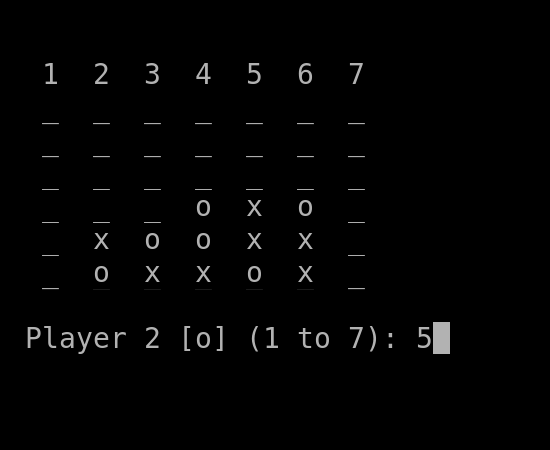
\includegraphics[width=0.5\linewidth]{pics/title.png}
    \begin{lstlisting}
        1 2 3 4 5 6 7                     1 2 3 4 5 6 7
        _ _ _ _ _ _ _                     _ _ _ _ _ _ _
        _ _ _ _ _ _ _                     _ _ _ _ _ _ _
        _ _ _ _ _ _ _                     _ _ _ _ O _ _
        _ _ _ o x o _                     _ _ _ O x o _
        _ x o o x x _                     _ x O o x x _
        _ o x x o x _                     _ O x x o x _

  Player 2 [o] (1 to 7): 5          Player 2 has won the game.
    \end{lstlisting}
\end{center}

\section*{Abstract}

«Vier gewinnt» ist ein weit verbreitetes und bekanntes Strategiespiel für zwei Personen, bei der es darum geht, vier Spielsteine auf einem 7x6-Raster in eine horizontale, vertikele oder diagonale Reihe zu bringen. Zu Zeiten der Corona-Krise lässt sich das Spiel schlecht in physischer Gegenwart an einem Tisch spielen. Ausserdem schaffen die altbekannten Spielregeln und -mechaniken kaum noch einen Anreiz für das Spiel. In der vorliegenden Arbeit soll das Spiel «Vier gewinnt» mit neuen Mechaniken interessanter und besonders auf die Personengruppe der Systemadministratoren angepasst werden, die das Spiel lieber auf der Kommandozeile als in der physichen Version spielen. Die Auswirkung dieser neuen Mechaniken werden im Rahmen eines \textit{Playtests} mit verschiedenen Versuchspersonen untersucht.
 
\newpage

\tableofcontents
\newpage

\section{Erste Iteration: Zieldefinition und Konzept}

Systemadministratoren (kurz: Sysadmins) haben es nicht einfach zu Zeiten der Corona-Krise: Ins Home-Office verbannt sind sie teilweise ihrer letzten sozialen Kontakte beraubt, zumal \textit{Star Wars}-Conventions und andere Veranstaltungen für Nerds alle abgesagt worden sind ‒ und dies auf eine lange Zeit hinaus. Als kleinen Trost sollen sie ein kleines Computerspiel bekommen, das im Rahmen dieses Projekts konzipiert und entwickelt wird. Dabei handelt es sich um eine erweiterte Version des Spiels «Vier gewinnt» (siehe \imgref{fig:vier-gewinnt}).

Sysadmins haben spezielle Bedürfnisse.\footnote{Als Sysadmins werden im Rahmen der vorliegenden Arbeit nur die Mitglieder der höchsten Kaste bezeichnet ‒ die Unix-Systemadministratoren. Auf die Bedürfnisse der Angehörigen tieferer Kasten soll hier nicht eingegangen werden.} Das herkömmliche «Vier gewinnt» ist ihnen zu langweilig, zumal sie sämtliche Speilverläufe schon längst nachtsüber auf einem ihrer High-End-Server durchgerechnet haben. Zudem ist ihnen nach Spielende das lästige Sortieren der Steine nach Farben, das beim «Vier gewinnt» im Meatspace nötig ist, ein Graus, zumal Sysadmins solche mechanischen Abläufe lieber automatisieren. Ausserdem lassen sich die Spielverläufe beim physischen Spiel nur sehr umständlich und schlecht maschinenlesbar festhalten, etwa mittels Fotokamera.

\begin{figure}
    \centering
    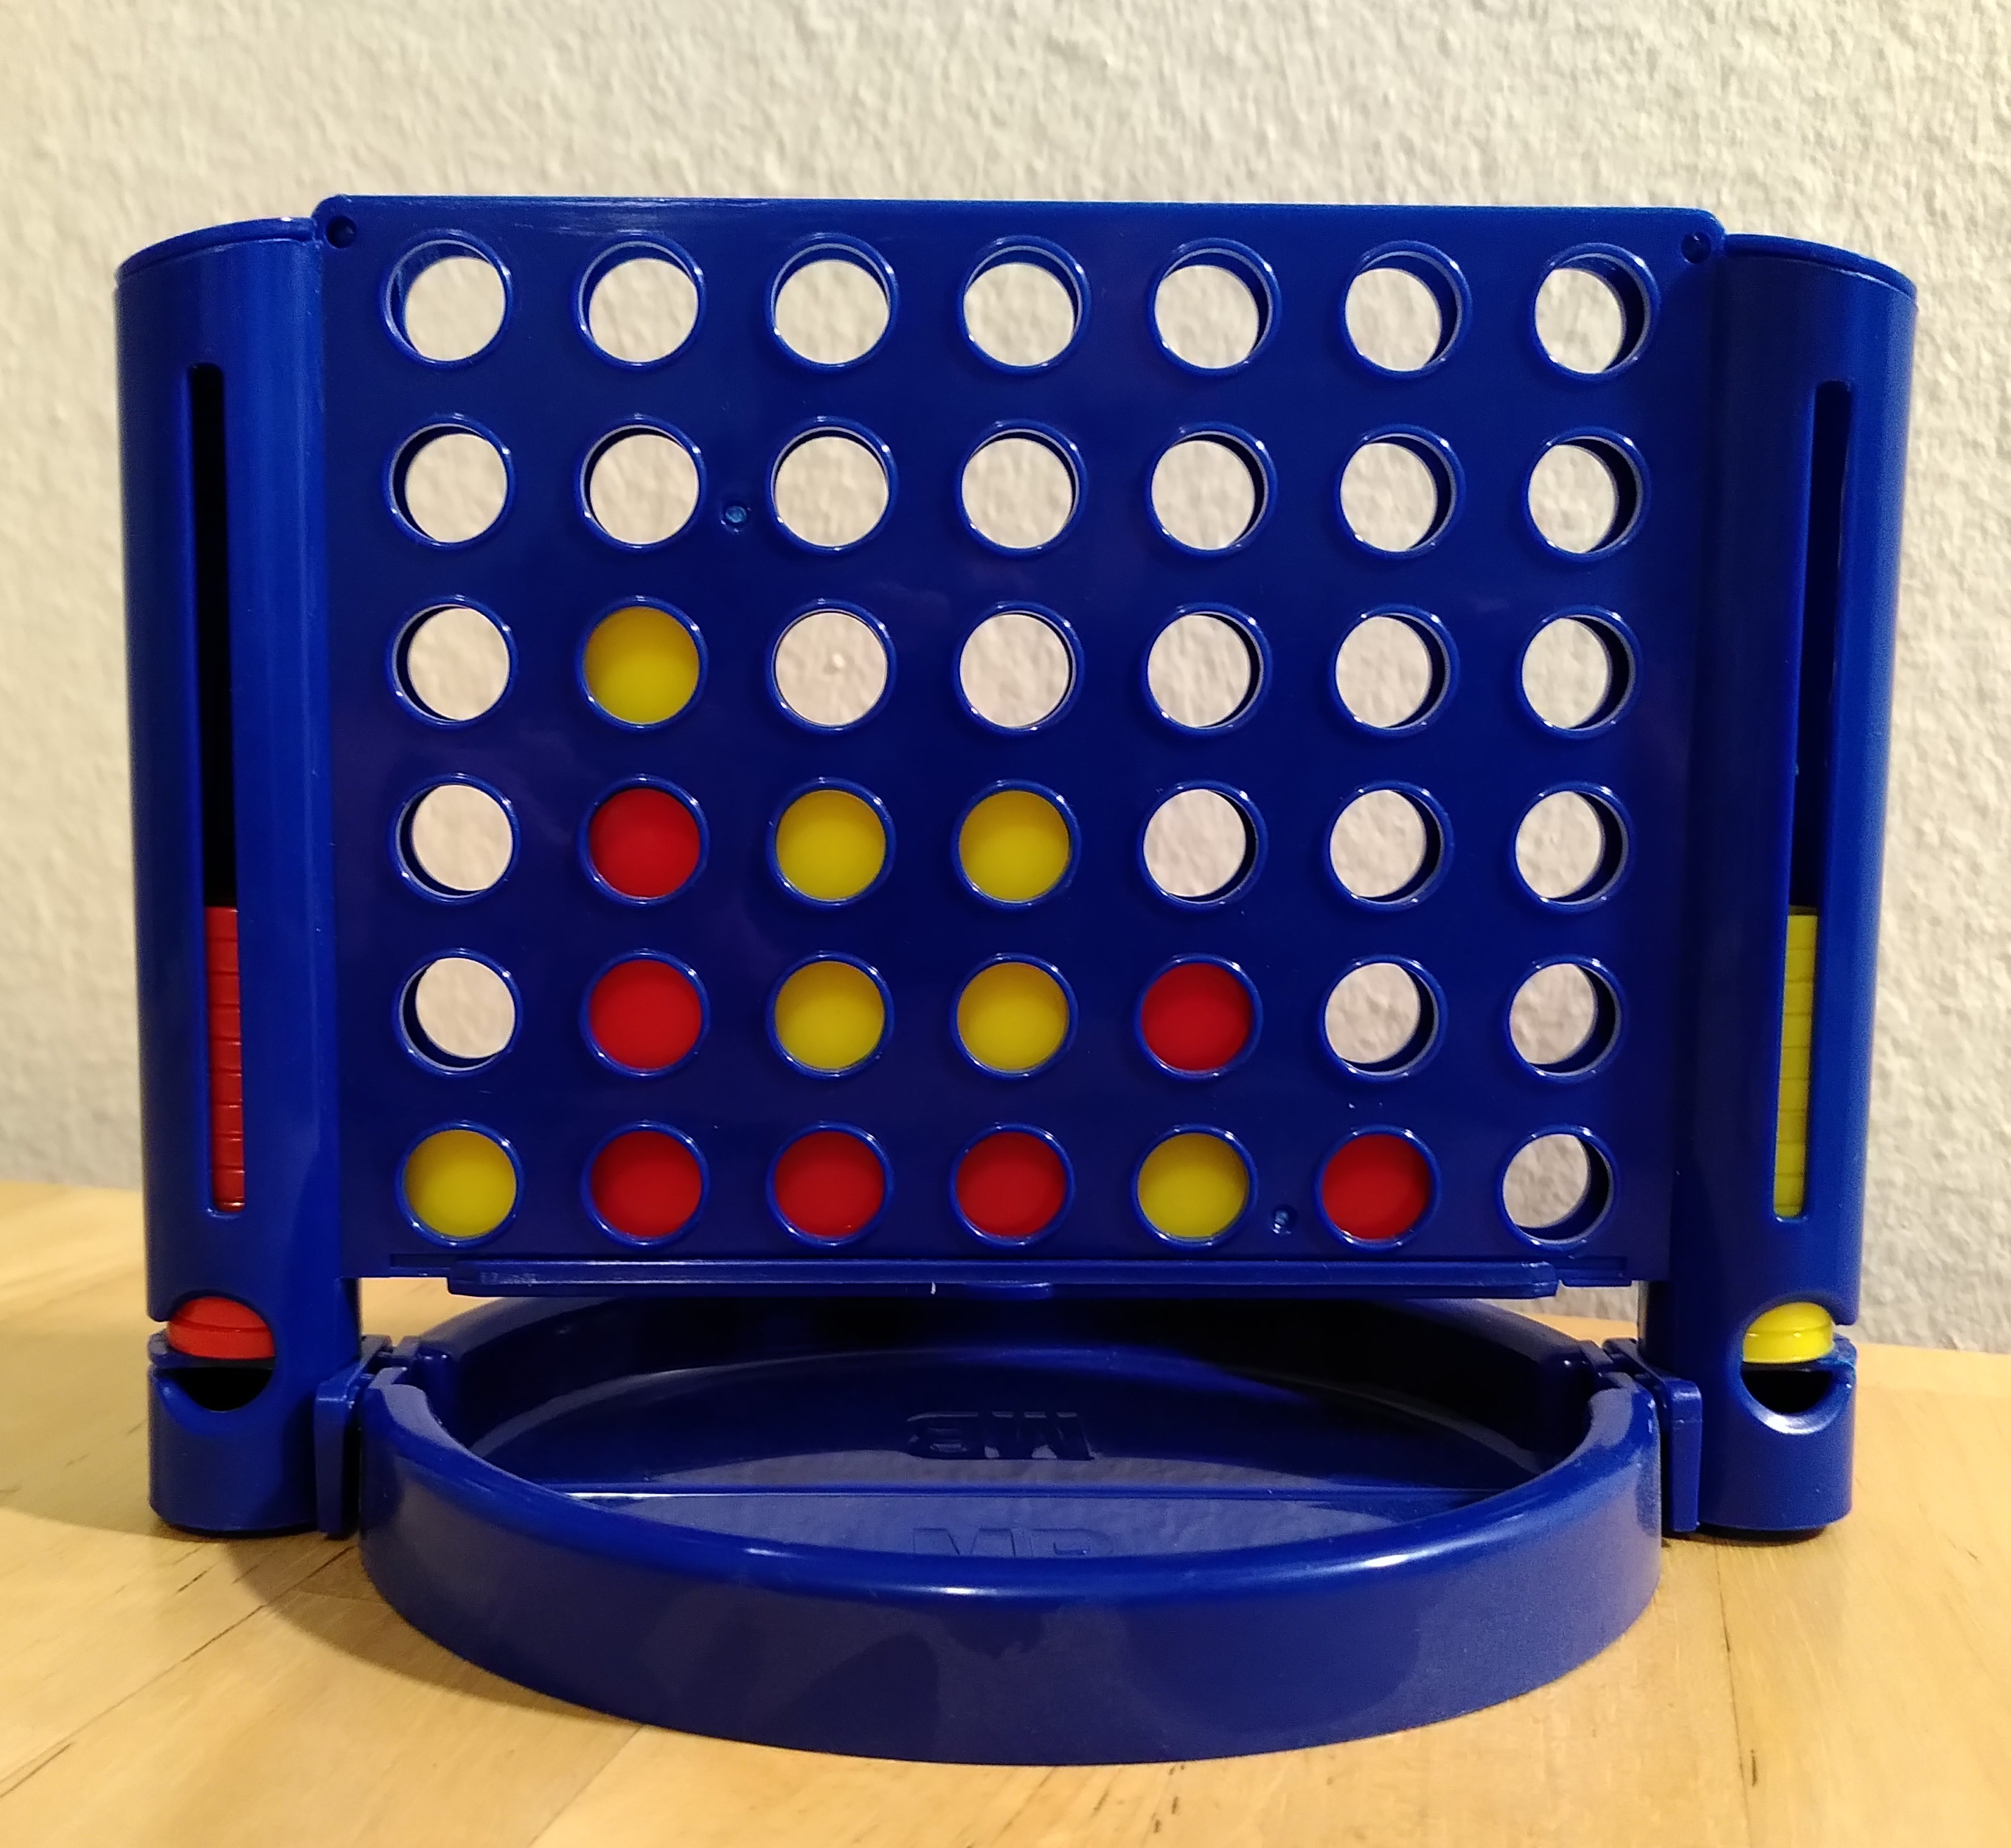
\includegraphics[width=1.0\linewidth]{pics/vier-gewinnt.jpg}
    \caption{Das klassische «Vier gewinnt» (Meatspace-Version). Die grellen Farben der VGA-Palette überfordern das auf die monochrome Bildschirmdarstellung optimierte Auge eines Sysadmins. Das analoge Einwerfen der Steine in die Schächte weckt traumatische Erinnerungen an die Handhabung einer Computermaus.}
    \label{fig:vier-gewinnt}
\end{figure}

\subsection{Vorteile der Kommandozeilenversion}

«Vier gewinnt» wäre viel besser, wenn man es auf der Kommandozeile spielen könnte! Dies hätte folgende Vorteile gegenüber der herkömmlichen Meatspace-Version:

\begin{enumerate}
    \item Das Spiel könnte während der Arbeitszeit gespielt werden, ohne dass der gelegentlich vorbei- und in den Bildschirm schauende Vorgesetzte diese Strategie der Arbeitsvermeidung als solche erkennen könnte. Schliesslich handelt es sich ja bloss um irgendwelche kryptisch anmutende Zeichen, die da auf dem Bildschirm zu sehen sind. Bestimmt hat der Sysadmin da einen Belegungsplan für Pins oder dergleichen auf dem Bildschirm, und selbstverständlich handelt es sich dabei um geistige Schwerstarbeit, die dem Arbeitgeber zugute kommt ‒ das verrät schon des Sysadmins angestrengter Gesichtsausdruck!
    \item Die Aufforderung der Geschäftsleitung, mehr zu kommunizieren und sich Probleme gemeinsam anzuschauen, könnte für weitere Arbeitsvermeidung ausgenutzt werden, indem sich zwei Sysadmins am gleichen Computer treffen, um dort «Vier gewinnt» (bzw. «v13rg3w1nn7») zu spielen. Die kryptisch anmutende Pin-Be\-le\-gung, die da für den Vorgesetzten auf dem Bildschirm zu sehen ist, schreit ja geradezu nach einer \textit{Pair Debugging Session}! So kann die Arbeitszeit weiter mit «Vier gewinnt» vertrödelt werden, und die sozialen Kontakte der Firma werden dadurch noch weiter gestärkt ‒ ganz im Sinne der Geschäftsleitung!
    \item Da solche sozialen Interaktionen im Meatspace derzeit wegen \textit{Social Distancing} kaum denkbar sind, müsste das Spiel auch remote von zwei Sysadmins spielbar sein, ohne dass die Nerds der Softwareentwicklung das Spiel aufwändig umprogrammieren müssen. So könnten die Sysadmins das Spiel von zu Hause aus über eine gemeinsame Session mit \texttt{tmux} oder GNU \texttt{screen} gegeneinander spielen. Dies dürfte auch die VPN-Verbindung ins Büro nicht weiter beeinträchtigen, zumal diese schon durch BitTorrent-Downloads voll ausgelastet ist. Der Multiplayer-Modus wäre somit auch über eine serielle Verbindung möglich, die der erfahrene Sysadmin notfalls auch aus im Büro gestohlenen Büroklammern und aus abgerissenen Streifen seines Aluhuts herstellen könnte. Sollte der Bildschirm des Sysadmins unerwartet in die Brüche gehen, wäre das Spiel immer noch über einen Fernschreiber spielbar, der sich bei jedem guten Systemadmin im Keller finden lässt.\footnote{In der Regel hinter der Kiste mit den \textit{Star Trek}-Fanartikeln.}
    \item Die Spielverläufe können einfach in Textdateien\footnote{d.h. MIME-Type \texttt{text/html;charset=utf-8}, selbstverständlich ohne \textit{byte order mark} (BOM)} festgehalten werden. Das erleichtert die Diskussion über Spielstrategien auf dem Usenet und in IRC.
\end{enumerate}

Das klassische «Vier gewinnt» müsste hierzu etwas interessanter ausgestaltet werden, sodass die Motivation der Sysadmins zumindest das Warten auf den nächsten Download auf den derzeit chronisch überlasteten Steam-Servern überdauert. Solche Verbesserungen sollen im Rahmen dieser Arbeit vorgeschlagen, umgesetzt und evaluiert werden.

\subsection{Zwei Tastaturen, eine Kommandozeile}

Um das Treffen zweier Sysadmins auf einem gemeinsamen Terminal, das für die Evaluation des Prototyps nötig ist, zu bewerkstelligen, muss ein gemeinsam zugänglicher Server zuerst entsprechend konfiguriert werden.\footnote{Server können von HSLU-Studierenden kostenlos und unkompliziert im \textit{Enterprise Lab} bezogen werden. Diese dürften knapp genügend Leistung aufbringen, um eine Anbindung mit einer Baudrate von 9600 über längere Zeit zu gewährleisten. Mit neueren Versionen von Solaris dürfte sich auch \texttt{tmux} einfach installieren lassen (siehe \url{https://www.opencsw.org/packages/tmux/}).}

Sollte wider aller Erwartung kein Solaris, sondern ein Debian-basiertes Betriebssystem auf dem Server installiert sein, lässt sich die gemeinsame Spielumgebung mit den folgenden Schritten einrichten.

Zunächst muss \texttt{tmux} installiert werden:

\begin{lstlisting}
# apt-get install tmux
\end{lstlisting}

Als nächstes ist eine gemeinsame Benutzergruppe und je ein Benutzer für die beiden Spieler (\texttt{geek} und \texttt{poke}) zu erstellen. Auch müssen den neu erstellen Benutzern gleich Passwörter hinterlegt werden:

\begin{lstlisting}
# groupadd sysadmins
# useradd -G sysadmins -m geek
# useradd -G sysadmins -m poke
# passwd geek
# passwd poke
\end{lstlisting}

Das \texttt{\$HOME}-Verzeichnis, das über das \texttt{-m}-Flag erstellt wird, ist wichtig, da die beiden Spieler ihre Spielverläufe ja schliesslich in Textdateien festhalten und kommentieren wollen ‒ letzteres vorzugsweise mit \texttt{ed(1)}, dem Standard-Texteditor von Unix.

Nun kann sich der erste Benutzer (\texttt{geek}) auf dem Server einloggen und eine neue \texttt{tmux}-Session namens \texttt{game} eröffnen:

\begin{lstlisting}
[geek]$ tmux -S /tmp/shared new -s game
\end{lstlisting}

Die Session muss so berechtigt werden, dass alle Benutzer der Gruppe \texttt{sysadmins} darauf zugreifen können:

\begin{lstlisting}
[geek]$ chgrp sysadmins /tmp/shared
\end{lstlisting}

Anschliessend kann sich der zweite Benutzer (\texttt{poke}) einloggen und an der bestehenden \texttt{tmux}-Session teilnehmen:

\begin{lstlisting}
[poke]$ tmux -S /tmp/shared attach -t game
\end{lstlisting}

Jetzt benötigen die beiden Spieler bloss noch ein Spiel, und der Spass kann auf einer tiefen Bandbreite beginnen!

\subsection{Prototyp für «Vier gewinnt»}

In dieser ersten Iteration soll nur das herkömmliche «Vier gewinnt»-Spiel zum Einsatz kommen. Dieses muss zunächst in einer Kommandozeilenversion entwickelt werden.

Als Umsetzungsplattform für den Prototyp kommt Python 3 zum Einsatz. Mit dieser Programmiersprache hat der Autor dieser Arbeit bereits einiges an positiver Erfahrung sammeln können. Ausserdem verfügt Python mit NumPy\footnote{\url{https://numpy.org/}} über eine mächtige Library für (mehrdimensionale) Arrays, mit der sich viele Listenoperationen mit wenig Code und effizient umsetzen lassen.\footnote{Für die richtige Version des Spiels würde eine Programmiersprache verwendet werden, die eine höhere Laufzeitperformance bei geringerem Speicherverbrauch ermöglicht, wie z.B. ANSI C 89, Assembler oder Fortran 66, damit der Sysadmin sich nicht unnötig Rechenpower für das Bitcoin-Mining verliert.}

Die Spiellogik wird mithilfe von pytest\footnote{\url{https://docs.pytest.org/en/latest/}} automatisiert getestet. Auch wenn es sich nur um einen Prototyp handelt, ist die Korrektheit der Spiellogik ein wichtiger Usability-Faktor, zumal nicht erkannte Gewinnsituationen für die Beteiligten sehr frustrierend sind, was einen negativen Einfluss auf die Testläufe hätte.

Der Prototyp ist einfach zu bedienen und schliesst Fehleingaben so gut wie möglich aus. Das Folgende Kommandozeilenfenster zeigt den Prototyp während eines bereits etwas fortgeschrittenen Spiels:

\begin{lstlisting}
        1 2 3 4 5 6 7
        _ _ _ _ _ _ _
        _ _ _ _ _ _ _
        _ _ _ _ _ _ _
        _ x _ _ o _ _
        _ o x o o o x
        _ x o x x x o

Player 1 [x] (1 to 7): ¶
\end{lstlisting}

Das Spielfeld wird mit einem 7x6-Raster dargestellt. Der Underscore (\texttt{\_}) markiert dabei leere Felder. Spieler 1 spielt mit dem Spielstein \texttt{x}, und Spieler 2 mit dem Spielstein \texttt{o}. Die Titelzeile markiert die einzelnen Spalten (oder «Schächte») mit einer Nummer, sodass sich der Spieler beim Auswählen des Schachts einfacher orientieren kann.

Das Paragraph-Zeichen (\texttt{¶}) markiert die Eingabeaufforderung. Der Spieler soll die Nummer des Schachts auswählen, in den sein Spielstein fallen soll. Falscheingaben (nicht numerische, nicht im Bereich 1-7, einen vollen Schacht bezeichnend usw.) werden nicht akzeptiert, sondern mit einer Fehlermeldung und einer erneuten Eingabeaufforderung quittiert:

\begin{lstlisting}
        1 2 3 4 5 6 7
        _ _ _ _ x _ _
        _ _ _ _ o _ _
        _ _ _ _ x _ _
        _ x _ _ o _ _
        _ o x o o o x
        _ x o x x x o

Player 2 [o] (1 to 7): 5
You must pick a free slot between 1 and 7!
\end{lstlisting}

Sind alle Spielfelder voll, ohne dass dabei ein Spieler die Siegbedingung (vier Spielsteine in einer horizontalen, vertikalen oder diagonalen Reihe) erfüllt, wird das Spiel als unentschieden gewertet. Erfüllt ein Spieler die Siegbedingung, ist das Spiel zu Ende und der Sieger wird als solcher ausgewiesen:

\begin{lstlisting}
        1 2 3 4 5 6 7
        _ _ _ _ x _ _
        _ _ _ _ o _ _
        _ _ _ _ X _ _
        _ x _ X o o _
        _ o X o o o x
        _ X o x x x o

Player 1 has won the game.
\end{lstlisting}

Hierbei wird zur leichteren Erkennung die Siegreihe hervorgehoben, indem der Spielstein durch einen entsprechenden Grossbuchstaben ersetzt wird (\texttt{x} wird hier durch \texttt{X} ersetzt). Dies soll Diskussionen zwischen aufbegrachten Sysadmins verhindern, die ansonsten nur in die Richtung gehen würde, dass diese Software halt falsch programmiert worden sei ‒ und die Erkennung der Siegbedingung nicht ausreichend getestet.

Das Spiel konnte in dieser Grundversion erfolgreich getestet werden. Es ist somit bereit für die Weiterentwicklung, die im nächsten Kapitel besprochen wird.

\newpage

\section{Zweite Iteration: Anwendung von Game-Design-Theorie}

In der zweiten Iteration soll das bestehende Spiel zunächst unter zwei verschiedenen theoretischen Aspekten des Game-Designs untersucht werden. Anschliessend sollen Vorschläge ausgearbeitet werden, wie das bestehende Spiel unter diesen beiden Gesichtspunkten verbessert werden kann.

\subsection{Theorie}

Beim Spielen von «Vier gewinnt» treffen die Spieler nur eine Art von Entscheidung: Die Wahl des Schachts, in welcher ein Stein eingeworfen wird. Auch kommt das Spiel ohne jegliche Zufallsmomente aus, wodurch es mit der Zeit etwas eintönig und ‒ beim wiederholten Spielen gegen den gleichen Kontrahenten ‒ mit der Zeit etwas absehbar wird. Bezogen auf das Spiel «Vier gewinnt» sollen darum diese beiden theoretischen Aspekte ‒ \textit{Entscheidungen} und \textit{Zufall} ‒ analysiert werden.

\subsubsection{Entscheidungen}

Verschiedene Spiele lassen verschiedene Arten von Entscheidungen zu. Bei einfachen Spielen hat man es v.a. mit uninteressanten Entscheidungen zu tun. Diese lassen sich in die folgenden Kategorien aufteilen:

\begin{description}
    \item[Keine Entscheidungen] Das Würfeln bei einem Leiterlispiel ist keine Entscheidung, da hier der Zufall regiert. Bei jeder Runde muss gewürfelt werden, der Spieler kann darüber nicht entscheiden.
    \item[Bedeutungslose Entscheidungen] Das Tippen auf Kopf oder Zahl beim Münzwurf ist eine bedeutungslose Entscheidung. Es muss eine Entscheidung getroffen werden, die das Spielergebnis aber nicht beeinflusst, bzw. vom Glück abhängig ist.
    \item[Offensichtliche Entscheidungen] Das setzen eines Steines in «Vier gewinnt» ist eine offensichtliche Entscheidung. Aus der Spielmechanik geht etwa klar hervor, welche Eröffnungszüge sinnvoll sind (in der Mitte spielen), oder welche Züge den Spieler dem Sieg näherbringen (Einreihung von Steinen).
    \item[Blinde Entscheidungen] Das Wählen einer Koordinate beim «Schiffe versenken» läuft zumeist blind ab, da man das Spielfeld des Gegners nicht kennt. Im Verlauf des Spiels erhält man jedoch immer ein besseres Bild vom Spielfeld des Gegners, sodass in manchen Spielsituationen das Versenken von grossen Schiffen zu einer offensichtlichen Entscheidung werden kann.
\end{description}

Beim Spiel «Vier gewinnt» hat man es mit offensichtlichen Entscheidungen zu tun. Umd as Spiel interessanter zu machen, muss es interessante Entscheidungen zulassen.

Interessante Entscheidungen unterscheiden sich von uninteressanten Enscheidungen u.a. dadurch, dass mit ihnen ein gewisses Risiko einhergeht, das sich nicht oder nur begrenzt abschätzen lässt. Oft wirken sich risikoreiche Entscheidungen nicht schon unmittelbar nach der Entscheidung, sondern erst später auf den Spielverlauf aus.

Bei «Vier gewinnt» steht dem Spieler nur eine Art von Auswahl zur Verfügung: Die Wahl des Schachts, in der ein Stein eingeworfen werden soll. Das Spiel kann dann interessanter werden, wenn andere Arten von Entscheidungen angeboten werden. Je nach Spielsituation wäre dann eine andere Art der Entscheidung angebracht.

\subsubsection{Zufall}

Der Zufall spielt in verschiedenen Spielen eine unterschiedlich grosse Rolle. Dabei lassen sich die Spiele in die folgenden Kategorien einteilen:

\begin{description}
    \item[Gewissheit] In einigen wenigen Spielen ist der Ausgang einer Partie schon im vorher so gut wie gewiss. Dies ist etwa im Spiel «Tic, Tac, Toe» der Fall, wo Partien in der Regel unentschieden enden ‒ sofern sich keiner der beiden Spieler extrem dumm anstellt.
    \item[Risiko] Bei sogenannten Glücksspielen, wie z.B. beim Roulette oder bei einarmigen Banditen, ist sich der Spieler über die Ungewissheit des Spielausgangs bewusst. Die Zufallskomponente entscheidet über Gewinn und Verlust.
    \item[Ungewissheit] Bei manchen Spielen gibt es keine Möglichkeit den Ausgang einer Partie vorauszusagen. Dies ist etwa in Spielen wie Schach der Fall, gerade wenn man den Gegner nicht kennt.
\end{description}

Bei «Vier gewinnt» gibt es keine Gewissheit darüber, wie das Spiel ausgehen wird. Je besser man einen Gegner jedoch kennenlernt, desto besser kann man sich auf dessen Strategien einstellen. Der Spielverlauf wird dadurch besser absehbar ‒ und mit der Zeit langweilig.

Im Modul \textit{Deep Learning for Games} wurden u.a. die Eröffnungszüge verschiedener Spiele (u.a. «Vier gewinnt») betrachtet. Wenig überraschend wurde dabei festgestellt, dass der erste Spieler den ersten Stein am besten in den mittleren Schacht einwirft. Beim Spiel unter erfahrenen Spielern dürfte die Eröffnung deshalb immer gleich ausfallen, wodurch die ersten paar Züge mit der Zeit recht mechanisch ausgeführt werden dürften.

Durch das Fehlen jeglicher Zufallskomponenten dürfte «Vier gewinnt» nach einigen Partien gegen den gleichen Gegner recht langweilig werden.

\subsection{Verbesserung des Prototyps}

Das Fehlen von interessanten Entscheidungen und Zufallsmomenten führen zu einer geringen Langzeitmotivation bei «Vier gewinnt». Diese kann erhöht werden, wenn diese beiden Aspekte ins Spiel eingebaut werden. Hierzu wurden zwei Ideen entwickelt: Die Rotation des Spielfelds und zufällig fallende, neutrale Steine.

\subsubsection{Rotation als interessante Entscheidung}

Bei «Vier gewinnt» bleiben gespielte Steine bis zum Spielende an ihrer ursprünglichen Position. Das Spiel wird so recht statisch. Jeder Spielzug hat nur Auswirkungen auf ein Feld. Dass Steine sich nicht seitlich bewegen oder nach oben wandern können ist den Regeln der Physik geschuldet. Die abgetrennten Schächte verhindern die Bewegung der Steine nach links oder rechts; die Schwerkraft verhindert das Wandern der Steine nach oben.

Da es sich bei der vorliegenden Umsetzung um ein Computerspiel handelt, können diese Einschränkungen etwas gelockert werden. Lässt man die starren Schächte weg, bzw. macht man sie durchlässiger, könnten die Steine bei einer Drehung des Feldes in eine andere Spalte (bzw. dann: Zeile) fallen. Die Schwerkraft könnte dabei ihre Wirkung behalten.

Das gedrehte Spielfeld ändert dadurch seine Dimension von 7x6 auf 6x7. Interessant ist, dass sich die Positionen der einzelnen Steine dabei \textit{relativ zueinander} ändern könnten. \imgref{fig:rotation} veranschaulicht dieses Prinzip.

\begin{figure}
    \centering
    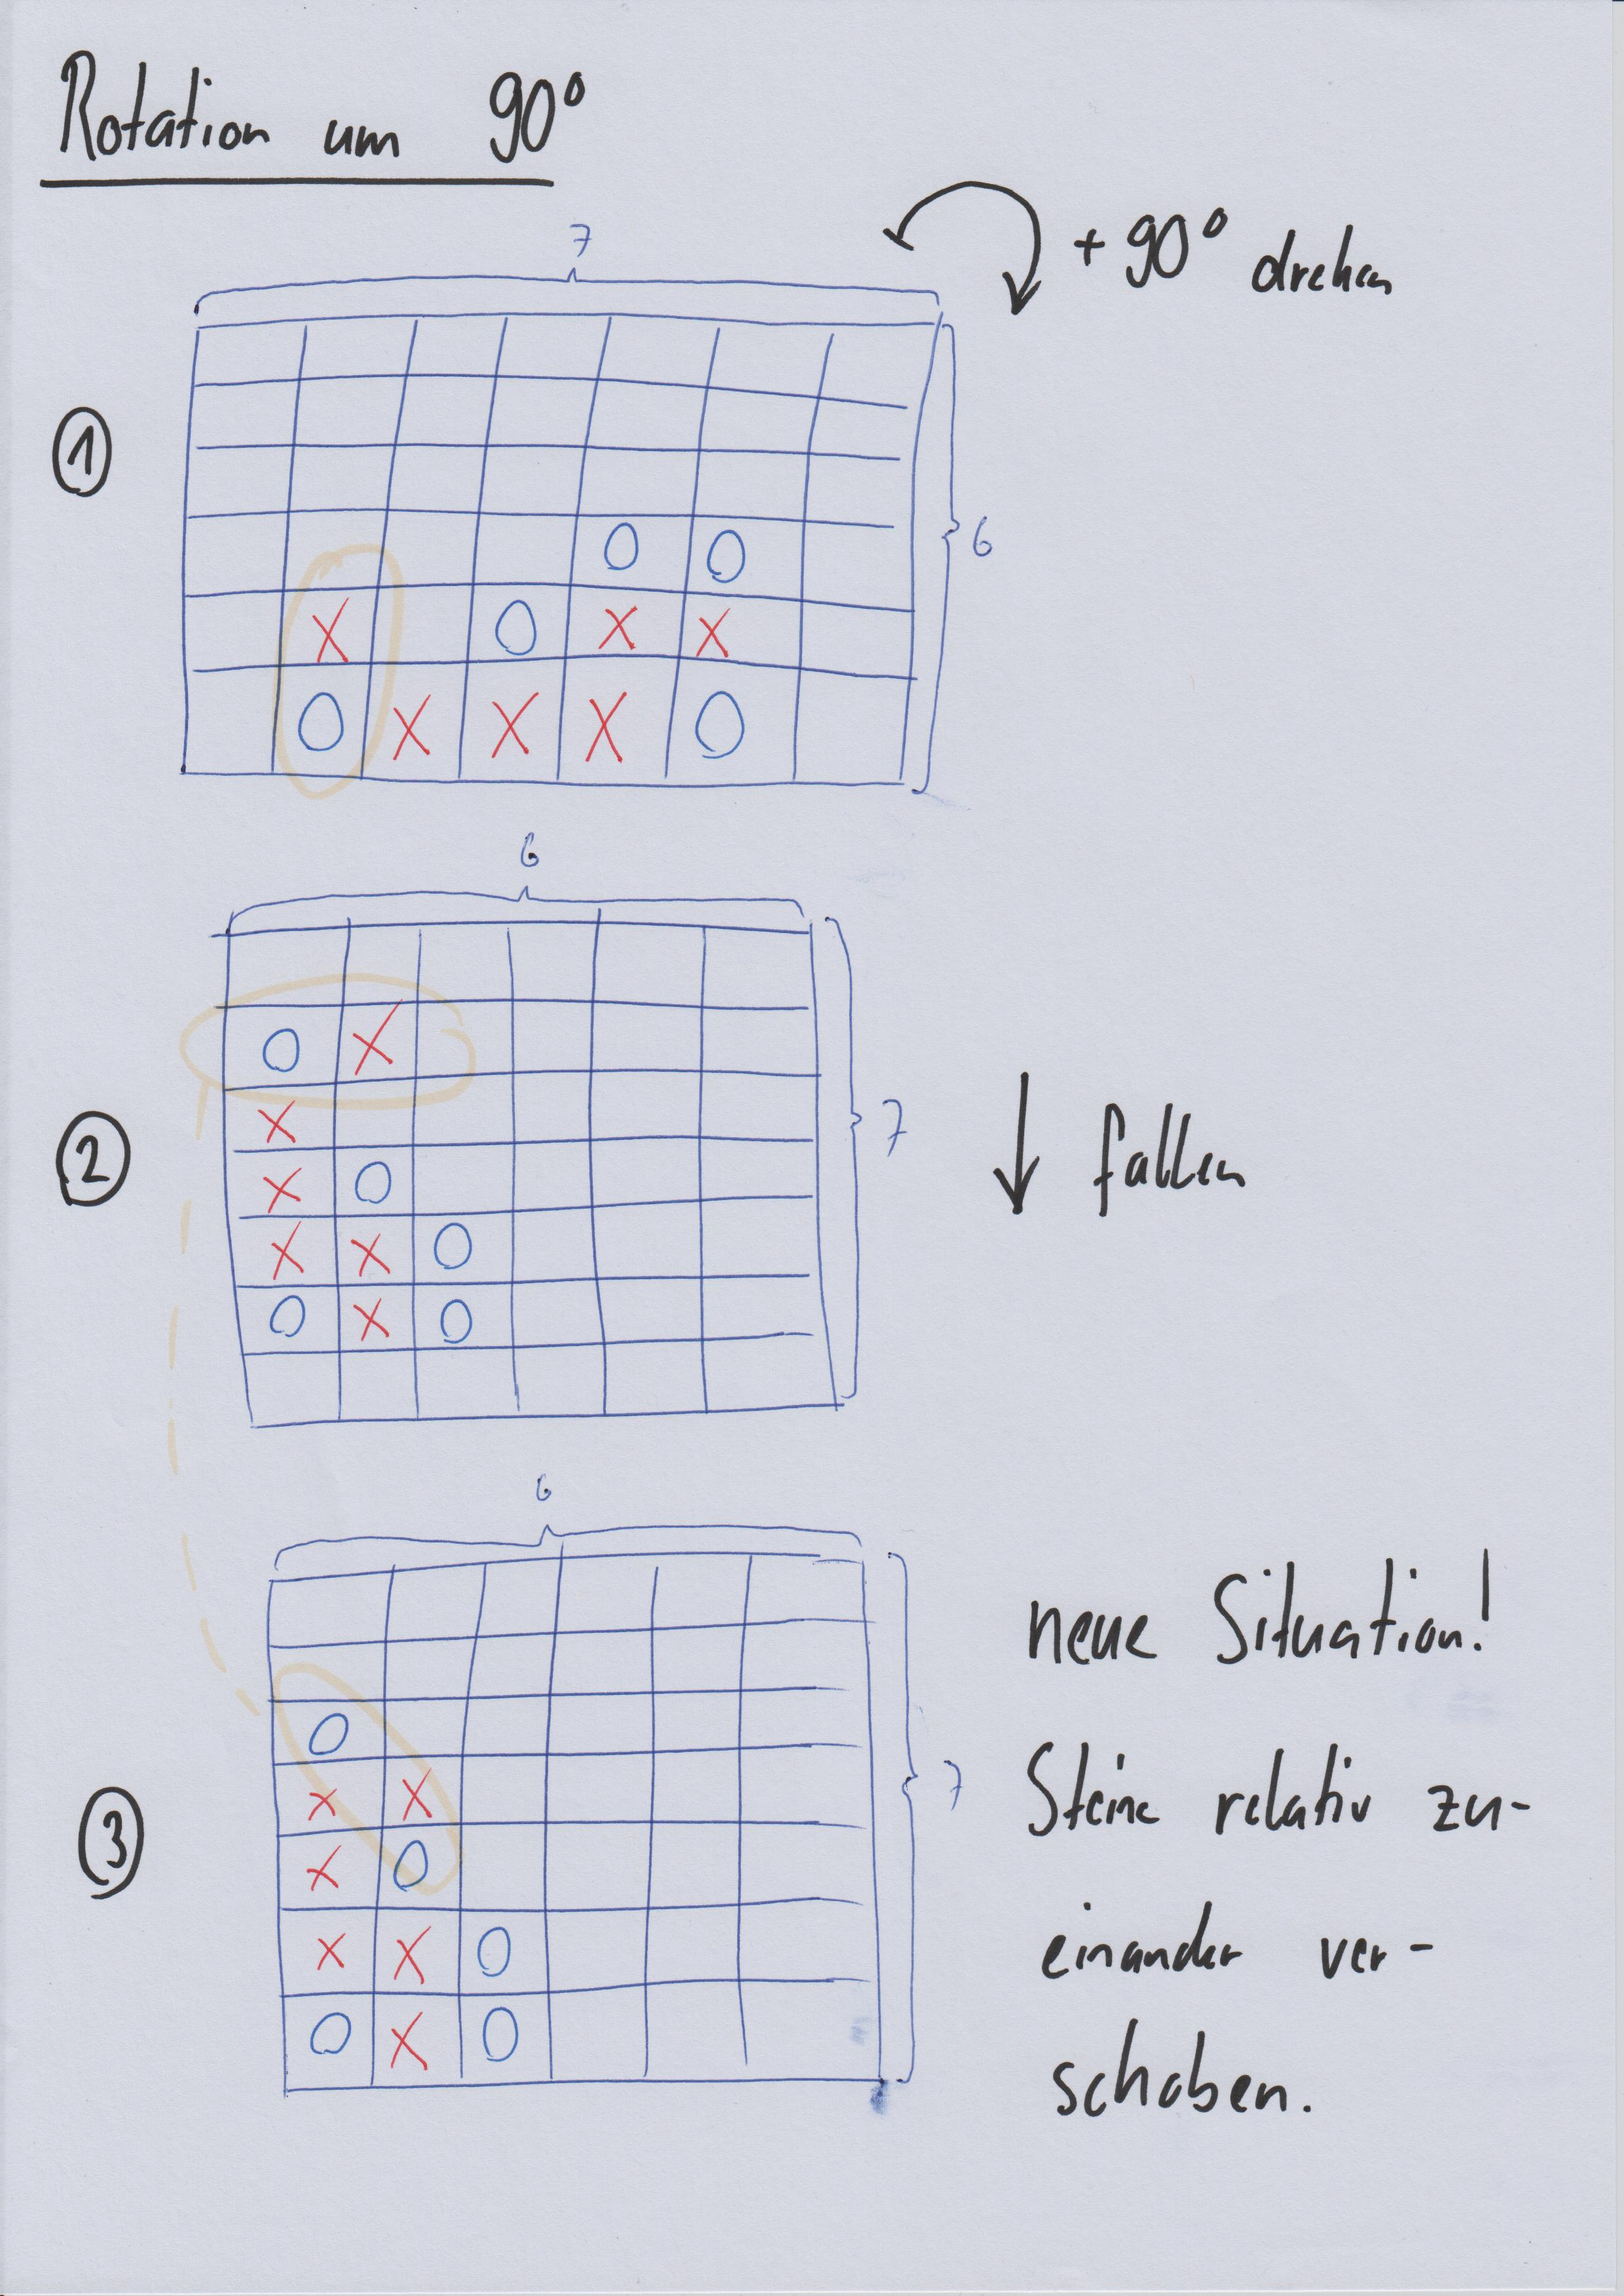
\includegraphics[width=0.9\linewidth]{pics/rotation-papier.jpg}
    \caption{Die Rotation um 90° als zusätzliche Spielmechanik. Das Spielgitter wird zunächst gedreht, anschliessend fallen die Steine nach unten. Dadurch entsteht eine neue Spielsituation, zumal sich manche Steine relativ zueinander bewegen.}
    \label{fig:rotation}
\end{figure}

Die Spieler sollen also die Möglichkeit erhalten, das Spielfeld zu drehen. Diese Aktion soll als Zug gelten, sodass der Spieler nach einer Drehung keinen weiteren Stein spielen kann, bis der Gegner seinen Zug (wiederum Drehung oder Stein spielen) ausgeführt hat.

Durch die veränderte relative Position der Steine zueinander kann sich so aufgrund einer Drehung eine Gewinnsituation ergeben. Es ist sogar möglich, dass hierdurch \textit{mehrere} Gewinnsituation ‒ eines oder gleich beider Spieler ‒ in einem Zug entstehen.\footnote{Der Einfachheit halber soll immer der Spieler als Gewinner gelten, der den letzten Zug vorgenommen hat. Das Gewinnen per Rotation erfordert viel Vorstellungsvermögen und ist somit ein kleiner Geniestreich.}

So kann ein Spieler mit einem guten Vorstellungsvermögen eine Situation herbeiführen, die für den Gegner unverdächtig aussieht, und nach einer Drehung des Spielfelds die Partie gewinnen. Selbstverständlich kann der Gegner diese Situation durch eine Drehung in die andere Richtung buchstäblich auf den Kopf stellen und so die Taktik seines Kontrahenten durchkreuzen.

Hierzu müssen zwei neue Spielzüge umgesetzt werden: Die Drehung des Feldes um 90° im Uhrzeigersinn (\texttt{rr} wie \textit{rotate right}) und im Gegenuhrzeigersinn (\texttt{rl} wie \textit{rotate left}).

Als Verfeinerung dieser Mechanik wäre es etwa denkbar, dass die Anzahl der Rotationen pro Spieler und Runde begrenzt oder erst nach einer bestimmten Anzahl gesetzter Steine erlaubt wären.

\subsubsection{Neutrale Steine als Zufallselement}

Da es beim wechselseitigen Setzen der Steine durch zwei Spieler keinen Zufall gibt, soll dieser über einen dritten (neutralen) Spieler eingefügt werden. Dieser wirft vor jeder Runde einen Stein in einen zufälligen (noch nicht komplett gefüllten) Schacht ein.

Dadurch ändert sich die Dynamik des Spiels von Beginn weg, zumal ein in der Mitte gesetzter neutraler Stein den idealen Eröffnungszug verunmöglicht. Fällt der erste zufällig platzierte Stein in die linke oder rechte Hälfte des Feldes, dürfte sich das Spiel tendenziell zunächst in der jeweils anderen Spielfeldhälfte entfalten.

Im weiteren Spielverlauf könnten dann Strategien einzelner Spieler durchkreuzt werden, indem ein zufällig fallender Stein den sicher geglaubten Sieg verhindert. Das Spiel wird dadurch neu lanciert. \imgref{fig:neutral} veranschaulicht die beiden genannten Auswirkungen auf die Spieldynamik.

\begin{figure}
    \centering
    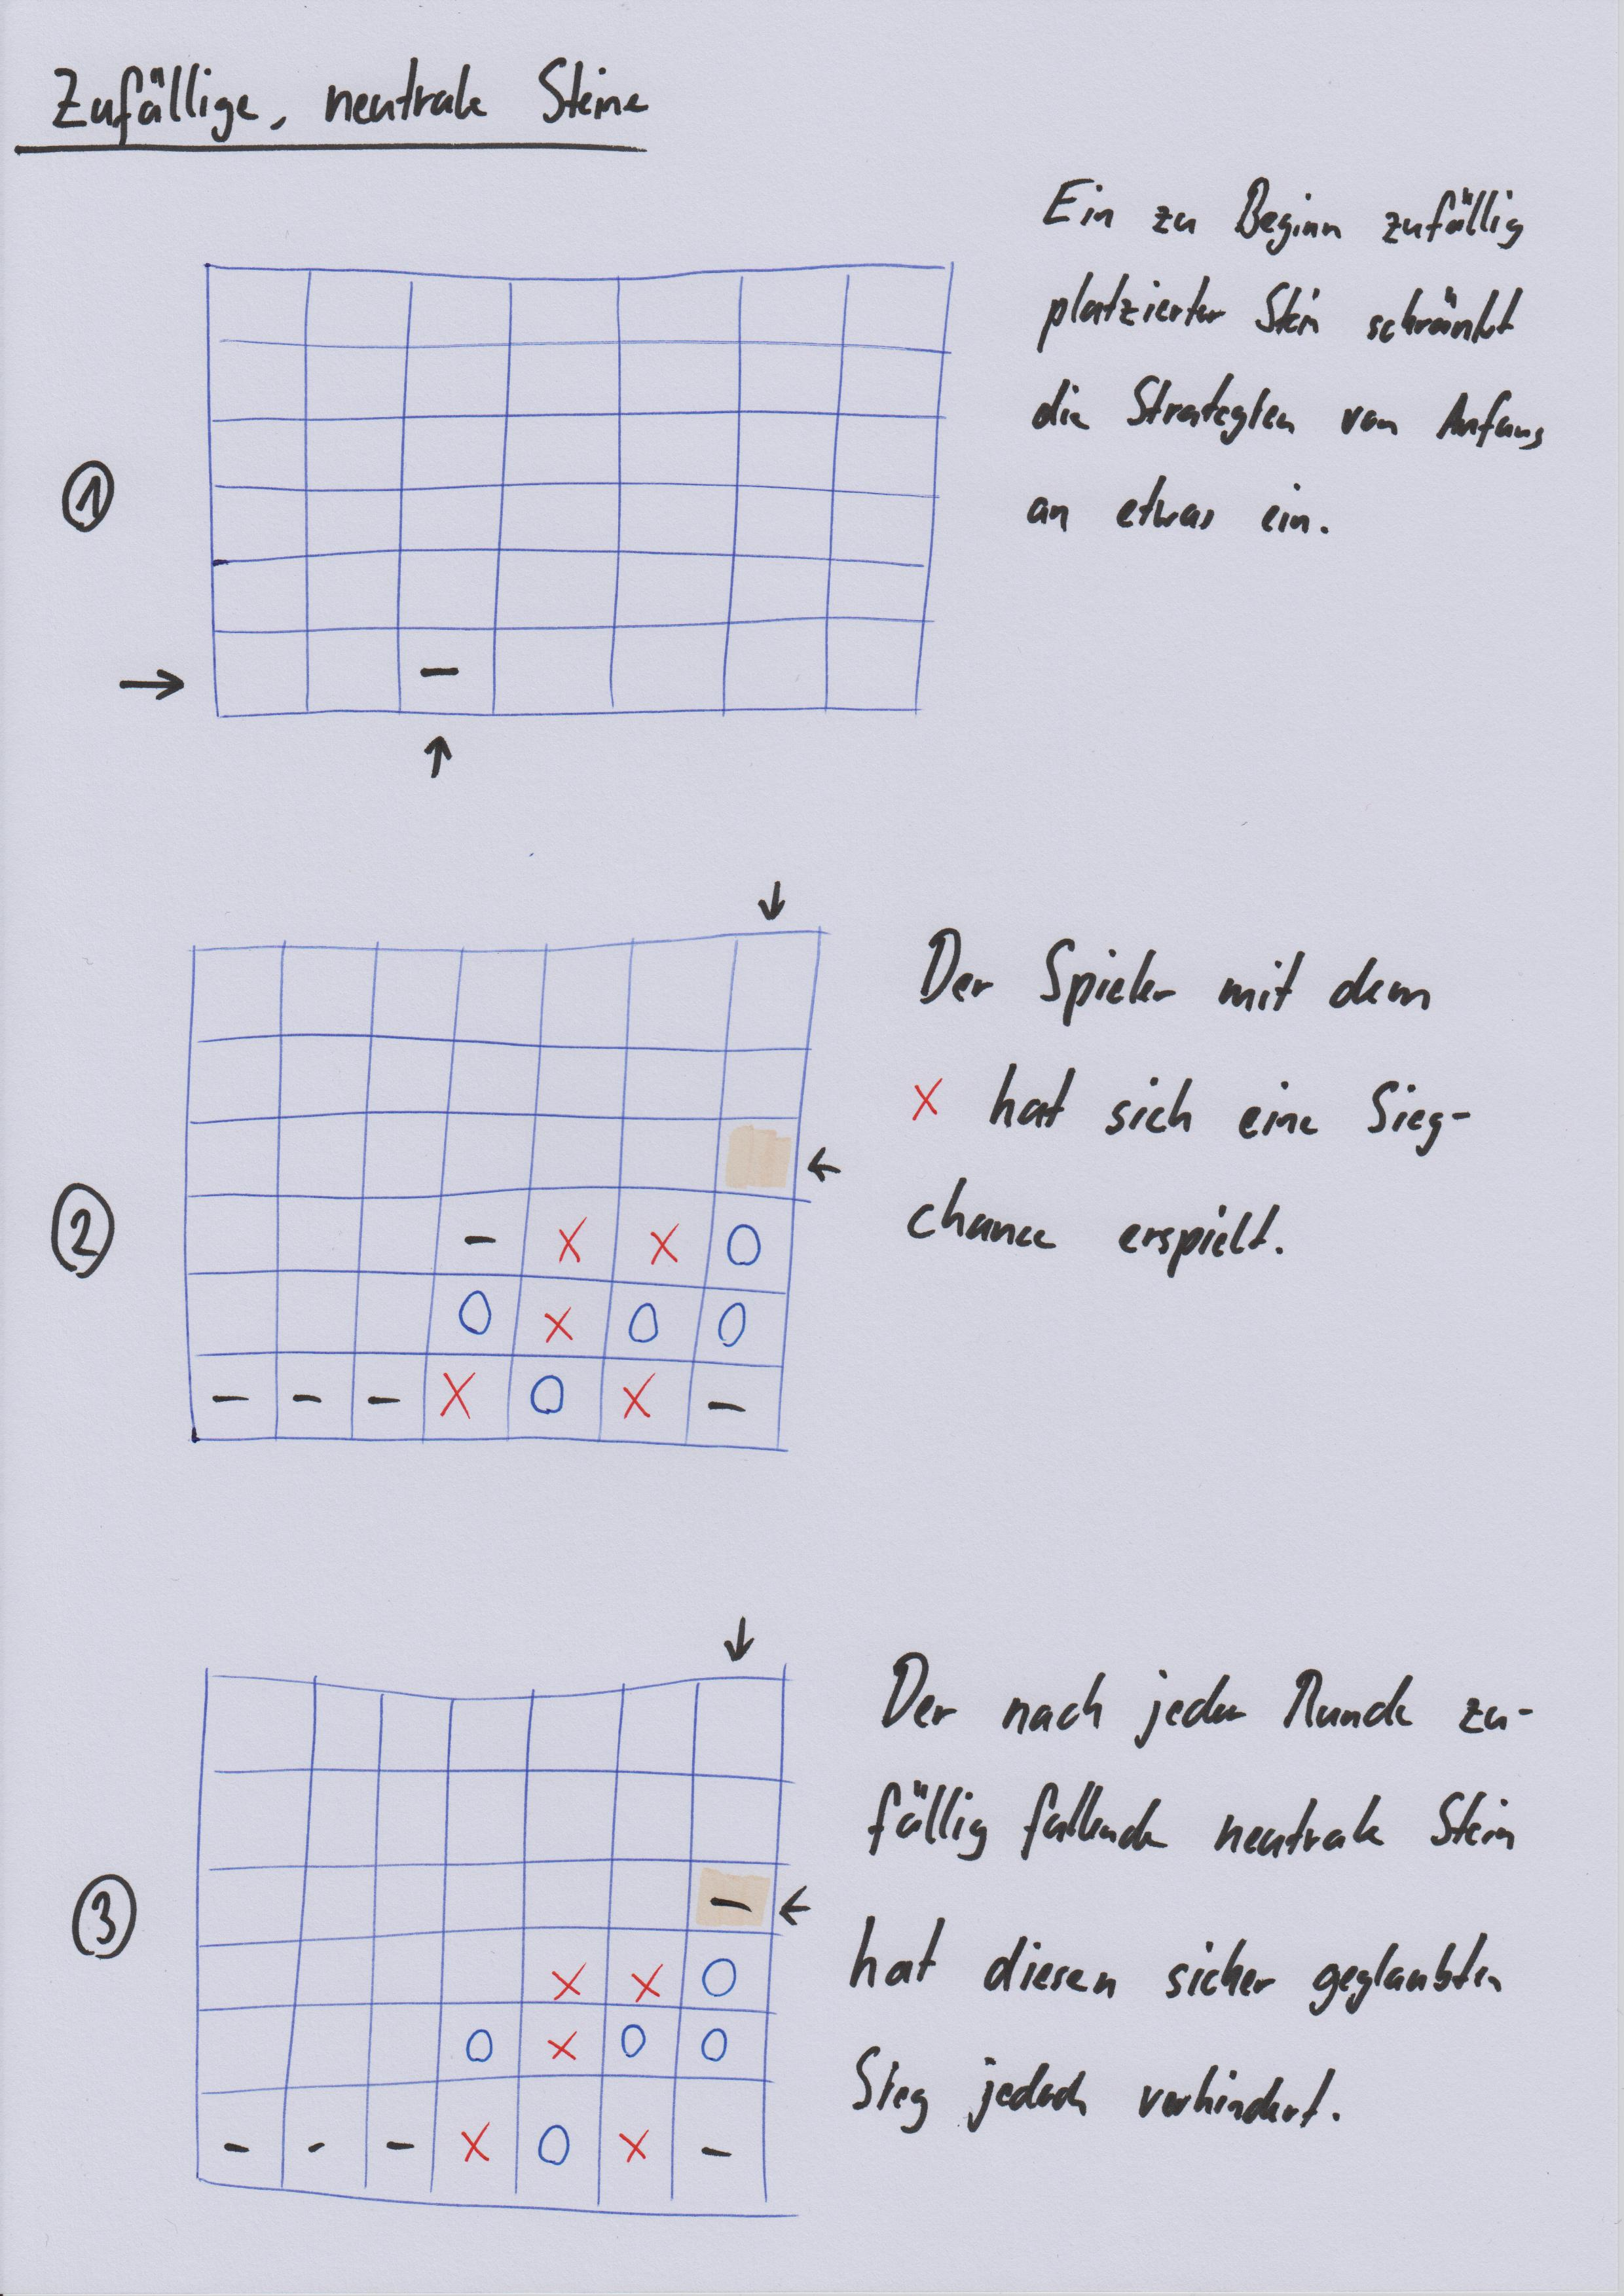
\includegraphics[width=0.9\linewidth]{pics/neutral-papier.jpg}
    \caption{Zufällig fallende, neutrale Steine sollen dem Spiel ein Zufallselement hinzufügen. Dadurch werden etablierte Strategien der Spieler möglicherweise durchkreuzt; sie müssen improvisieren.}
    \label{fig:neutral}
\end{figure}

Der beschriebene Ansatz könnte verfeinert werden, indem ein neutraler Stein nicht vor jeder Runde mit Gewissheit, sondern mit einer bestimmten Wahrscheinlichkeit fallen würde. Weiter wäre es möglich, \textit{mehrere} zufällige, neutrale Steine pro Runde mit einer bestimmten Wahrscheinlichkeit fallen zu lassen. Frequenz und Anzahl der Zufallssteine könnten dabei mit einer Wahrscheinlichkeitsverteilung definiert werden.

Durch den zusätzlichen dritten Spieler füllt sich das Spielfeld tendenziell schneller. Darum dürften die Partien aufgrund dieser Modifikation tendenziell öfters unentschieden ausfallen. Ein grösseres Spielfeld könnte hier Abhilfe schaffen.

\clearpage

\section{Dritte Iteration: Abschliessender Nutzertest und Reflexion}

Für die dritte Iteration, d.h. für den interaktiven Test des erweiterten Spiels, wurden die beiden beschriebenen Zusatzmechanismen jeweils in ihrer einfachsten Form entwickelt. Die vorgeschlagenen Verfeinerungen können dann als Ausblick aufgegriffen werden, sollten sich die umgesetzten Änderungen als unbefriedigend herausstellen.

\subsection{Spielen mit Zusatzfeatures}

Die beiden Zusatzfeatures können über ein Flag aktiviert werden:

\begin{description}
    \item[\texttt{--rotate}] Aktiviert die Rotation um 90° als zusätzliche Spielzüge. Mit \texttt{rr} wird das Spielfeld um 90° «nach recht» (\textit{rotate right}, im Uhrzeigersinn), mit \texttt{rl} wird das Spielfeld um 90° «nach links» (\textit{rotate left}, im Gegenuhrzeigersinn) rotiert.
    \item[\texttt{--neutral}] Aktiviert zusätzliche neutrale Steine. Eins solcher wird vor jeder Runde in einen zufälligen Schacht eingeworfen.
\end{description}

Die Beiden Optionen können kombiniert werden. Das Spiel wird dann folgendermassen aufgerufen (ausgehend vom Root-Verzeichnis des Repositories):

\begin{lstlisting}
$ cd src/
$ python -m venv env
$ source env/bin/activate
$ pip install -r requirements.txt
$ v13r93w1nn7/game.py --rotate --neutral
\end{lstlisting}

Ein möglicher Spielverlauf mit zufälligen, neutralen Steinen (Spielstein \texttt{.}) könnte inmitten der vierten Runde etwa so aussehen:

\begin{lstlisting}
        1 2 3 4 5 6 7
        _ _ _ _ _ _ _
        _ _ _ _ _ _ _
        _ _ _ _ _ _ _
        _ . x o _ _ _
        _ x . . _ _ _
        _ o x o x _ .

Player 2 [o] (1 to 7, rr/rl for rotation): rr
\end{lstlisting}

Spieler zwei entscheidet sich für eine Rotation um 90° im Uhrzeigersinn, was folgende Auswirkungena auf das Spielfeld hat:

\begin{lstlisting}
        1 2 3 4 5 6
        _ _ _ _ _ _
        _ _ _ _ _ _
        o _ _ _ _ _
        x _ _ _ _ _
        o x . _ _ _
        x . x _ _ _
        . . o _ . _

Player 1 [x] (1 to 6, rr/rl for rotation):
\end{lstlisting}

Man beachte, dass die Wahlmöglichkeiten der Schächte nun von vormals eins bis sieben auf neu eins bis sechs eingeschränkt worden sind.

Das Spiel ist somit weiterentwickelt worden und bereit für die Testläufe.

\subsection{Durchführung der Tests}

Das entwickelte Spiel soll mit mindestens drei Versuchspersonen gespielt werden, um eine gewisse Bandbreite an Rückmeldungen zu erhalten.

Zunächst soll mindestens eine Partie mit der ursprünglichen Version gespielt werden, d.h. das Spiel wird ohne die beiden eingeführten Optionen gestartet. Weitere Partien können angehängt werden um mit dem Setup und der Bedienung besser vertraut zu werden.

Anschliessend wird mindestens eine Partie mit dem \texttt{--neutral}-Flag gespielt. Kann die Versuchsperson die Auswirkung dieser Erweiterung nicht feststellen oder nicht artikulieren, sollen weitere Partien gespielt werden.

Es folgt mindestens eine Partie nur mit dem \texttt{--rotate}-Flag. So können die beiden Zusatzfeatures isoliert voneinander getestet werden.

Zum Schluss wird mindestens eine Partie mit beiden Flags, \texttt{--neutral} und \texttt{--rotate}, gespielt, um festzustellen, ob die \textit{Kombination} der beiden Erweiterungen andere Auswirkungen auf das Spiel hat als die beiden Erweiterungen für sich betrachtet. Wirken sich die beiden neuen Mechanismen wechselseitig aufeinander aus, oder ist die Auswirkung derselben bloss im Sinne der «Summe ihrer Teile» zu betrachten?

\subsection{Rückmeldungen der Spieler}

Die Rückmeldungen der Testpersonen nach den beschriebenen Testläufen lautete folgendermassen:

\begin{description}
    \item[Ksenia B.] Die Bedienung war zunächst bei der Grundversion nicht ganz verständlich. Nach den ersten paar Zügen bereitete dies jedoch keine Probleme mehr. Bei der Grundversion sei der Spielverlauf recht einfach absehbar. Der neutrale Spielstein (\texttt{.}) konnte zunächst optisch schlecht erkannt werden. Der Sieg wurde durch einen neutralen Stein ermöglicht, der nach einem Zug von Spieler 2 gefallen war. Man müsse also nicht nur darauf achten, wo der Gegner spielt, sondern auch, wo nach zwei Zügen jeweils ein neutraler Stein falle. Bei der Rotation hatte die Erkennung der Gewinnsituation zunächst nicht funktioniert.\footnote{Dies lag daran, dass Spieler 2 durch eine Rotation Spieler 1 zum Sieger gemacht hatte, wobei Gewinnsituationen immer nur für den Spieler ausgewertet wurden, der den letzten Zug machte. Dieses Verhalten ist für die Grundversion korrekt, musste aber im Zusammenhang mit der \texttt{--rotate}-Erweiterung angepasst werden (siehe Commit \texttt{e012a9e}). [Zwischen den Testläufen sollen nur schwere Fehler korrigiert werden. Anpassungen, die sich auf die Spielmechanik auswirken, werden unterlassen.]} Es benötige einiges an Vorstellungskraft um die Auswirkungen einer Drehung abschätzen zu können. So ist das Spiel aufgrund einer Rotation des Gegners entschieden worden. (Dessen Versuch ging nach hinten los.) Das Spiel mit der Kombination von \texttt{--rotate} und \texttt{--neutral} wurde ebenfalls durch eine Drehung entschieden, dieses mal aber vom Spieler, der die Drehung ausgeführt hatte. Dieser konnte die Situation jedoch nicht voll durchblicken, sodass der Sieg durch die Drehung ein Glückstreffer war. Insgesamt wurde der Drehmechanismus als positiv, wenn auch als herausfordernd bewertet. Die zufälligen, neutralen Steine kamen schlecht weg, denn dadurch verkomme das Spiel zu einem Glücksspiel. Auch sei das Feld dafür etwas zu klein und fülle sich zu schnell an. Drehungen sind durch die Zufallssteine noch schwieriger abzuschätzen, da mehr Steine beachtet werden müssen.
    \item[Maurin D. T.] Die Bedienung war von Anfang an verständlich. Die Darstellung war etwas klein, doch daran gewöhnte man sich nach einigen Zügen. Nach einer Testrunde mit der Grundversion wurden die neutralen Steine dazugeschaltet. Diese machten das Spiel etwas interessanter, aber auch anspruchsvoller, da man auf einen zusätzlichen «Mitspieler» achten müsse. Das Feature wurde eher als Ablenkungsfaktor denn als weitere taktische Möglichkeit gewertet, denn es machte eher Strategien kaputt als neue zu ermöglichen. Beim Test mit der Rotation wurde diese zunächst als etwas irritierend empfunden, da die Drehrichtung zu Beginn nicht ganz klar war. Nach einigen Spielzügen war dies jedoch geklärt, und es wurden viele Drehungen ausgeführt. Diese könne einem taktische Vorteile bringen und mache es besonders einfach, das Konzept des Gegners zu zerstören, wodurch sie zu einer destruktiven Spielweise verleite. Weiter antizipiere man eher die Auswirkung einer Rotation als sich auf die aktuelle Position der Steine zu konzentrieren und diese zu analysieren. Impulsive Spieler könnten die Rotation gut als Verlegenheitszug nutzen. Die Rotation selber war in keiner Runde der siegbringende Zug, lenkte aber von der Taktik der Spieler ab, sodas sie indirekt zum Spielausgang beitrug. Die Kombination von neutralen, zufälligen Steinen und der Rotation wurde als irritierend empfunden. Ein destruktives Spiel mit ständigen Drehungen eines Spielers lässt in der Regel den Gegner gewinnen, da dieser schlicht mehr Steine setzen könne: destruktive Strategien führen so ins Abseits. Konstruktive Strategien würden durch die zufälligen Steine erschwert. Die Variante mit der Rotation wurde insgesamt als die interessanteste empfunden. Die Rotation bringe neue strategische und taktische Möglichkeiten und mache das Spiel interessanter.
    \item[Carli B.] Nach einigen Verbindungsproblemen funktionierte das Spiel tadellos, und die Bedienung war sofort verständlich. Die Grundversion wurde für eine Runde gespielt. Beim Spielen mit den zufälligen, neutralen Steinen wurden gleich zu Beginn Bedenken geäussert, dass dies zu vielen Unentschieden führen könne. Der Mechanismus wurde als unfair beurteilt, da Spieler 2 nicht direkt auf die neutralen Steine reagieren könne, und Spieler 1 dadurch einen Vorteil erhalte. Der Punkt (.) als Darstellung für die neutralen Steine wurde negativ bewertet, da er vertikal nicht in der Mitte, sondern eher unten zu liegen kommt. Als nächstes wurde die Rotation ausprobiert, indem zunächst das Feld einige Male mit wenigen Steinen hin und her rotiert worden war. Bei einer Runde hat sich eine Siegchance aufgrund einer Drehung ergeben, die dann aber nicht genutzt worden ist. Bei der Neuorientierung nach der Drehung ist nämlich für \textit{beide} Spieler eine Siegchance entstanden, und der erste Stein nach der Drehung wurde genutzt, um des Gegners Spiel zu sabotieren, statt die eigene Siegchance zu nutzen. In einer weiteren Runde kam es zu einer Rotation, die dem Gegner zu einem Sieg verhalf: Die Auswirkung der Drehung wurde nicht korrekt antizipiert. Bei der Kombination der zufälligen, neutralen Steine mit der Drehung war es recht schwierig zu gewinnen. Hier hat wiederum eine Drehung zu einer Position geführt, von der aus im nächsten Zug gewonnen werden konnte. Eine weitere Runde endete unentschieden. Unterm Strich wurden die neutralen Steine eher negativ bewertet. Es wäre besser, wenn diese nur mit einer Wahrscheinlichkeit von ungefähr 30\% pro Runde erscheinen würden. Ansonsten hätte man zu wenig Platz für die Spielentfaltung. Der Vorschlag, das Feld zu vergrössern, wurde auch als sinnvolle Variante bewertet. Weiter wurde vorgeschlagen, statt neutrale Steine zufällig zu setzen, bestehende Steine nach dem Zufallsprinzip zu entfernen. Dies wäre aber schwer darstellbar. Am besten ist die Variante mit der Rotation angekommen. Die Auswirkungen einer Drehung seien zwar schwer abzuschätzen, aber mit der Zeit auch lernbar. So könne man sich im Spiel laufend verbessern. Die Zufallssteine wurden negativ bewertet, da das Spiel mit ihnen zu einem Glücksspiel verkomme. Beim Poker bestehe zwar auch eine grosse Zufallskomponente, diese beeinflusse aber v.a. die Ausgangslage, weniger den Spielverlauf. Mit den Zufallssteinen sei es für einen guten Spieler unnötig schwierig das Spiel zu gewinnen.
\end{description}

\subsection{Fazit}

Die beiden Erweiterungen arbeiten in entgegengesetzte Richtungen: Belohnt der Drehmechanismus eine hohe Vorstellungskraft und ermöglicht neue Strategien, verkommt das Spiel mit den zufällig fallenden, neutralen Steinen zu einem Glücksspiel. Für letztere sei das Feld ‒ wie befürchtet ‒ etwas zu klein.

\newpage

\listoffigures
\addcontentsline{toc}{section}{Abbildungsverzeichnis}

\end{document}
